% to render
% pdflatex [ filename ] && pdflatex [ filename ]

\documentclass{article}
% \documentclass[twocolumn]{article}


\usepackage{graphicx}
\usepackage{amsmath, amsthm, amssymb}
\usepackage{parskip}

% block code
\usepackage{alltt}

% set margins
\usepackage[margin = 1in]{geometry}
\setlength{\parindent}{1cm}

\usepackage{setspace}
% for double spacing the entire document
% \doublespacing
\singlespacing

% fancier captions
\usepackage{caption}
\captionsetup[figure]{font = small, labelfont = small}

%% imported packages
\usepackage{paralist}

% reference tables and figures, in the style of eqref
\newcommand{\figref}[1]{Fig. (\ref{#1})}
\newcommand{\tabref}[1]{Table (\ref{#1})}

% stylistic shortenings
\newcommand{\ti}[1]{\emph{#1}}
\newcommand{\tb}[1]{\textbf{#1}}
\newcommand{\cpart}[1]{\newblock{\LARGE {\\\\#1}}}
\renewcommand{\arraystretch}{1.3}

% comments that should be hidden
\newcommand{\comment}[1]{}

% note syntax
\newcommand{\note}[1]{\newblock{\small [ \ti{\tb{#1}} ]}}
% hide notes
% \newcommand{\note}[1]{\comment{#1}}

% inline code
\newcommand{\code}[1]{\texttt{$\text{#1}$}}

% vector stylization
\newcommand{\vect}[1]{\boldsymbol{#1}}
% \newcommand{\vect}[1]{\vec{#1}}

\begin{document}
% small text
% \small

\title{\tb{Parallel Load Balancing}}
\author{Minke Zhang\hspace*{-\tabcolsep}}
\date{\today}

% make title
\begingroup
\let\center\flushright
\let\endcenter\endflushright
\maketitle
\endgroup

\section{Modules}

\cpart{Lamport Queue}

The lamport queue will export the following functions--

\begin{alltt}
struct lamport_queue_t \{
  int size;
  Packet_t **elem;
  ...
\} q;

q *q_init(int depth);
void enq(q *q, Packet_t *pkt);          // called only by the dispatcher thread
Packet_t *deq(q *q);                    // called only by the parent worker thread
int is_full(q *q);
int is_empty(q *q);

\end{alltt}

\cpart{Workers}

Each worker is responsible for processing data from one source, which is stored in the associated queue--
\begin{alltt}
struct worker_t \{
  int p_remaining;                        // packets which have yet to have been supplied
                                          //   by the dispatcher
  q *q;
  int is_done;                            // !p_remaining && is_empty(q)
  ...
\} worker;

worker *init_worker(int q_depth, int T);  // initializes the worker and the associated queue
void *execute_worker(void *args);         // thread handler for the worker
long process_packet(worker *);            // blocks until w->q is not empty and processes
                                          //   next packet

\end{alltt}

\cpart{Dispatcher}

The dispatcher thread is responsible for relaying data from the provided \code{packet\_source\_t} provider--

\begin{alltt}

struct dispatcher_t \{
  worker **workers;                       // list of worker data structs
  ...
\} dispatcher;

dispatcher *init_dispatcher(...);
void *execute_dispatcher(void *args);     // thread handler for the dispatcher
                                          // loops through the list of workers and assigns
                                          //   non-full queues with an appropriate packet
                                          // skips fully-queued workers
                                          // exits when sum(w->is_done) equals the number
                                          //   of workers

\end{alltt}

\cpart{Executable}

The main executable should have the following format--

\begin{alltt}

struct result_t \{
  float time;                             // the main return result
  long fingerprint;                       // the fingerprint of the data generated -- used for
                                          //   correctness testing
  ...
\}

result *(*firewall_execute) (int T, int n, long W, int is_uniform, short id);

\end{alltt}

\section{Hypotheses}

\tb{NB}: we define \ti{speedup} $\sigma$ in this document as the relative execution speed of the respective execution method versus the serial (reference) 
implementation. Thus, if we say that the speedup of implementation $X$ was $0.8$, we are stating that implementation $X$ is slower than the serial implementation 
under identical executable parameters $\mathcal{P} = (n, T, D, W)$.

\cpart{Parallel Overhead}

As was the case with the Floyd-Warshall parallel implementation, we would expect a certain \code{pthread} overhead generated-- the relative contributing factor of 
the overhead however, will depend on how much time the executable will spend processing actual packet data. As such, we would expect that $\sigma$ would approach 
unity as $W \to \infty$ and as $n \to 1$.

\cpart{Dispatcher Rate}

Here we are testing the efficiency of the dispatcher when tasked with distributing packets across multiple workers. In the case that a worker queue is full, the 
expected behavior of the dispatcher is to skip over the worker and attempt to distribute the appropriate packet to the next worker-- as the \code{worker} data 
structure has the \code{p\_remaining} property which counts the number of packets still left from the global packet number, the dispatcher can simply refuse to 
decrement the counter and will know to add extra packets to the appropriate worker once the queue is free.

If the dispatcher is fully parallelized, we expect that the throughput to increase linearly with the number of threads. However, due to the serial nature of the 
dispatcher, we will expect an asymptotic falloff away from the linear relationship as $n \to \infty$.

\cpart{Speedup with Uniform Load}

The worker rate represents work which is parallelizable, whereas the dispatcher rate represents work which cannot be parallelized. We can thus use Ahmdal's law to 
approximate the expected speedup as a function of thread count. However, we expect that the expected speedup is an \ti{upper} bound to the measured curve, as thread 
overhead is nontrivial in the cases to be tested.

\cpart{Speedup with Exponentially Distributed Load}

We would expect the speedup to be significantly less than the serial implementation, as the load imbalance would mean unlucky threads are spending far more time 
over their equally-distributed number of packets than the threads with lower tids.

\section{Data \& Analysis}

\cpart{Parallel Overhead}

\begin{figure}
\begin{center}
	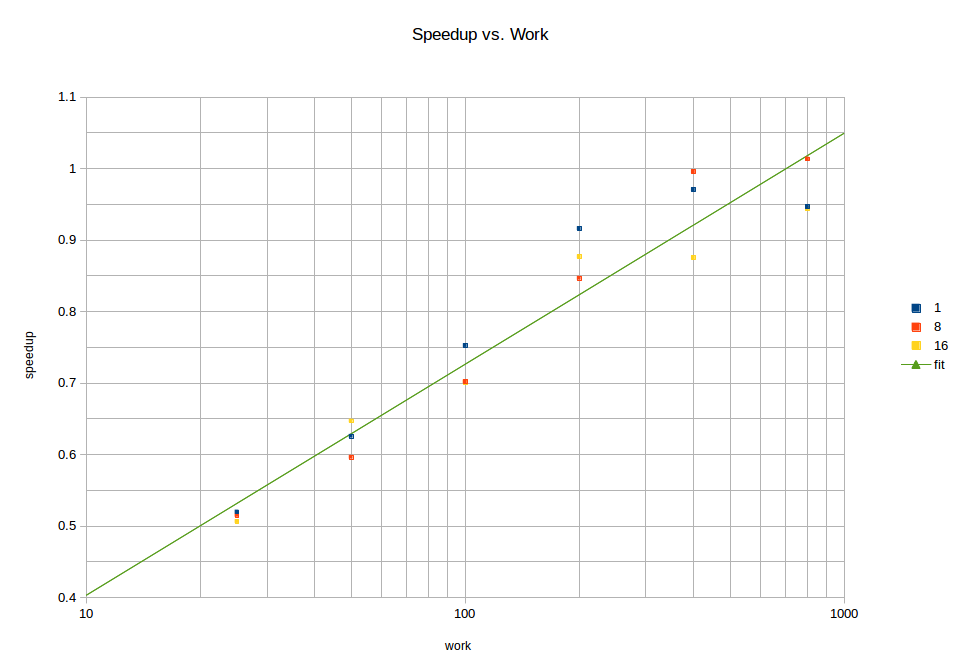
\includegraphics[scale=0.5]{speedup_vs_work.png}
	\caption{The parallel overhead is demonstrated by comparing the running time of \code{serial\_queue} vs. \code{serial}. As more time is spent on processing the packet (work), we see the parallel data struct overhead contribute to less of the running time.}
	\label{speedup_vs_work}
\end{center}
\end{figure}

\begin{figure}
\begin{center}
	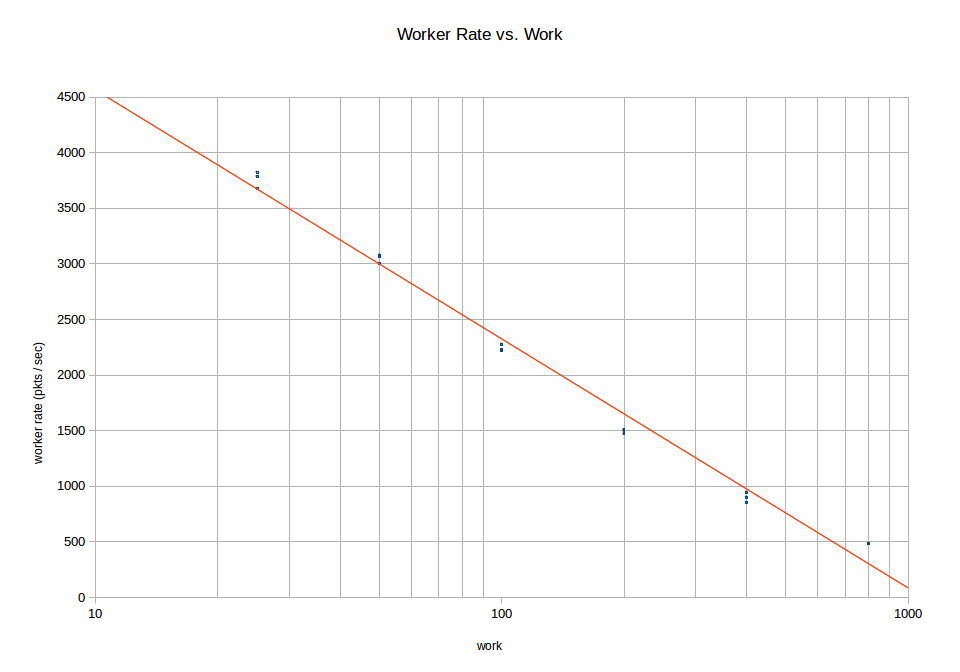
\includegraphics[scale=0.5]{worker_rate.png}
	\caption{Total packets processing rate is plotted against the work involved with processing each packet. Line of best fit $$wR(W) = 0.1404\text{ ln}(W) + 0.0797$$}
	\label{worker_rate}
\end{center}
\end{figure}

We see that the relative speedup of the serial queue implementation (representing the parallel overhead) increases towards unity as $W \to \infty$, as is expected-- 
the relative amount of work done by \code{getFingerprint} increases as $W$ increases, which leads to the overall decreased contribution of time allotted in 
initializing the parallel data structures.

\cpart{Dispatcher Rate}

\begin{figure}
\begin{center}
	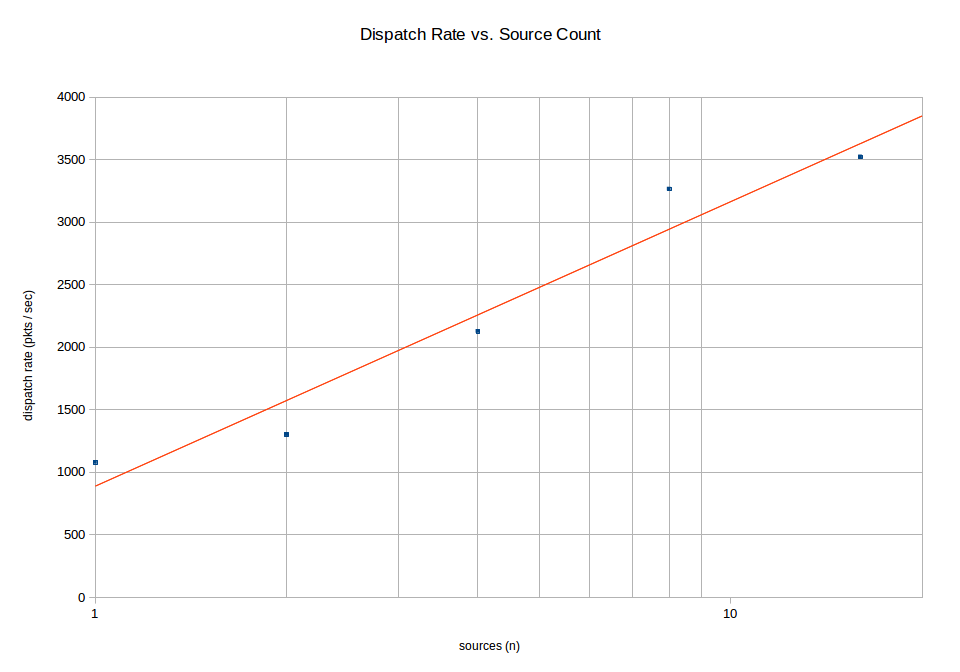
\includegraphics[scale=0.5]{dispatcher_rate.png}
	\caption{Packet rate being dispatched as a function of the number of threads. We see that the rate levels off (as is the characteristic of a logarithmic function) as $n \to \infty$. Line of best fit $$dR(n) = 987.8244\text{ ln}(n) + 890.3917$$}
	\label{dispatcher_rate}
\end{center}
\end{figure}

The dispatch rate represents the rate at which the dispatcher thread is able to hand out packets to the workers; we see that the logarithmic nature of the graph 
implies there are diminishing returns for increasing the number of threads, as the serial nature of the dispatch thread means we cannot process packets faster than 
the dispatcher can hand out-- the bottleneck here limits the fundamental utility of our program.

\cpart{Speedup with Uniform Load}

\begin{figure}
\begin{center}
	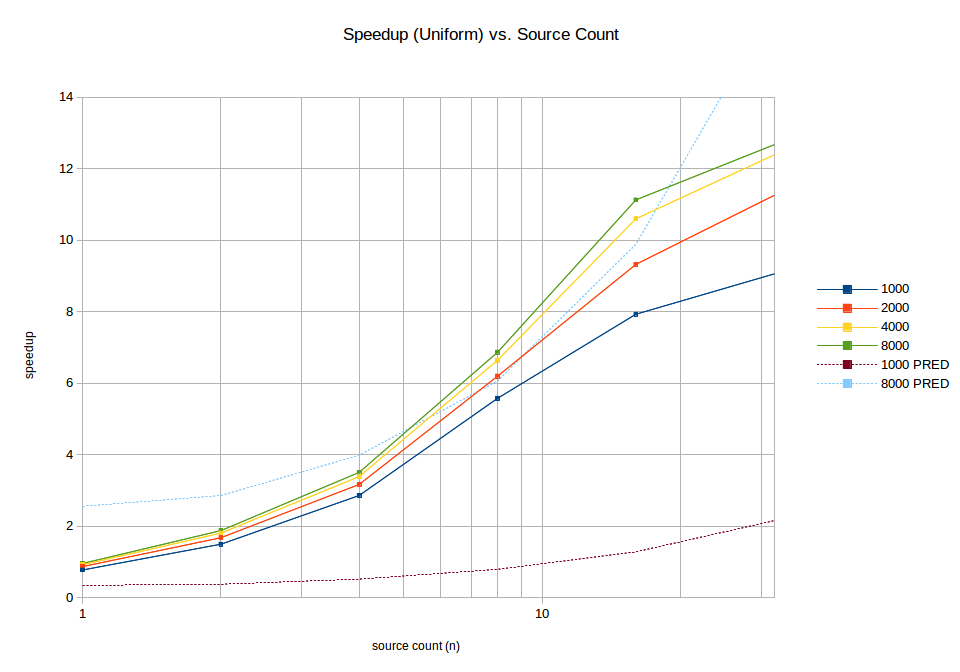
\includegraphics[scale=0.5]{uniform_speedup.png}
	\caption{Parallel execution speedup (uniform packet distribution) as a function of source count.}
	\label{uniform_speedup}
\end{center}
\end{figure}

We see that the spread of speedup ranges at $n = 32$ is much wider than the spread at $n = 1$-- this is expected, as the total amount of time spent in the 
$getFingerprint$ call becomes a significant portion of the running time of the program for high $W$, which as a result, benefits more parallelization.

Given the dispatcher rate $dW$ and the worker rate $rW$, the max rate at which packets can be processed is $\min(rW(W), dW(n))$; plugging the appropriate values of 
$W$ and $n$, we arrive at the predicted speedups as shown by the dotted lines in \figref{uniform_speedup}.

\cpart{Speedup with Exponentially Distributed Load}

\begin{figure}
\begin{center}
	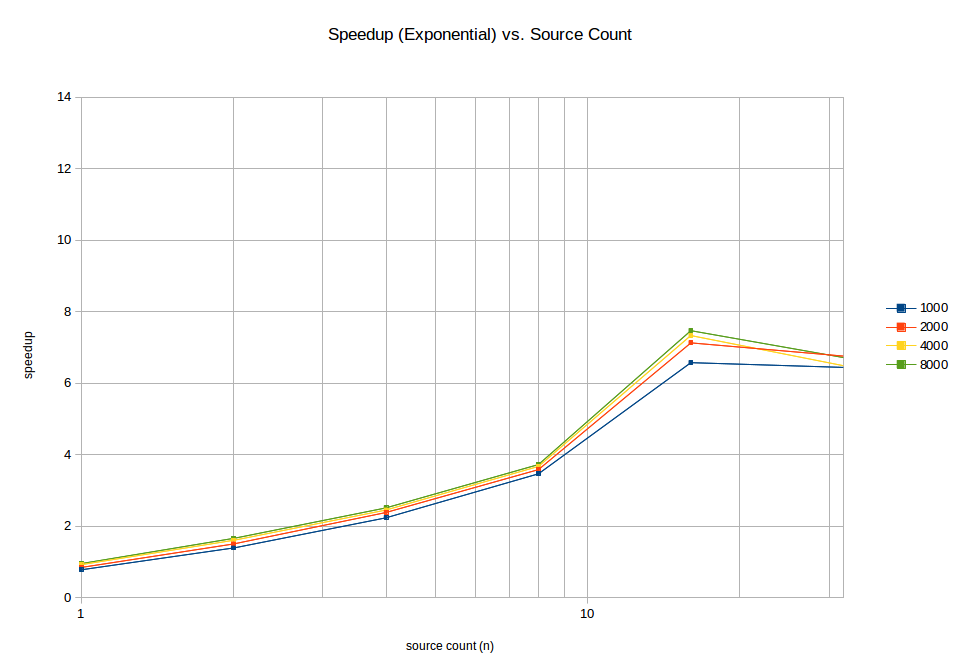
\includegraphics[scale=0.5]{exponential_speedup.png}
	\caption{Parallel execution speedup (exponential packet distribution) as a function of source count.}
	\label{exponential_speedup}
\end{center}
\end{figure}

Comparing \figref{exponential_speedup} with \figref{uniform_speedup}, we see that the speedup rates for an exponentially-distributed workload to be much less than 
that of the uniformly-distributed workload-- at $n = 16$, the relative speedup ratio between exponential and uniform distributions is $\sim77.8\%$; furthermore, we 
see that the relative speedup ratio is $\sim70\%$ at $n = 32$. This is to be expected, as was stated in the hypothesis, as load balancing in our parallel implementation cannot 
handle the workloads given to us.

\section{Testing}

\cpart{Queue Integrity}

We would like to ensure that the queue can be safely modified simultaneously by an enqueuing thread and a dequeuing thread-- as such we would like to implement a 
simple test model--

\begin{alltt}
struct blob_t \{
  q *q;
  Packet_t packets[DIM];
\} blob;

typedef void *(*func) (void *) thread_handler

void test_q(thread_handler) \{
  pthread_create(..., thread_handler, ...);
  for(int i = 0; i < DIM; i++) \{
    Packet_t p = deq(b->q);
    ASSERT(getFingerprint(p->...) == getFingerprint(b->packets[i]->...));
    ...
  \}
\}

void *enq_handler(void *args) \{
  blob *b = (blob *) args;
  for(int i = 0; i < DIM; i++) \{
    q_enq(b->q, b->packets[i]);
  \}
  ...
\}

void *enq_handler_sleep(void *args) \{
  blob *b = (blob *) args;
  for(int i = 0; i < DIM; i++) \{
    enq(b->q, b->packets[i]);
    sleep(1);
  \}
  ...
\}
\end{alltt}

\cpart{Packet Distribution}

The packets generated by calls within the dispatcher are initialized with the destination worker id as an input-- we can thus test packet distrubution by
\begin{enumerate}
	\item generate packets using exponential workload,
	\item assign the \ti{wrong} packets (that is, the hardest packets to a thread which should otherwise expect an easy load),
	\item use \code{stopwatch} to clock the execution times of each thread,
	\item see if the expected (wrong) thread is hit with a performance loss
\end{enumerate}

\cpart{Worker \& Dispatcher Quality Assurance}

We will use the fingerprints of the processed results to identify if the results given are correct; we will check \code{parallel\_firewall} and \code{serial\_queue\_firewall} against the results of \code{serial\_firewall}--

\begin{alltt}

void *test_correctness(void *args) \{
  ...
  result *p = serial_firewall(t, n, w, uniform_flag, i);
  result *q = parallel_firewall(t, n, w, uniform_flag, i);
  result *r = serial_queue_firewall(t, n, w, uniform_flag, i);
  ASSERT(p->fingerprint == q->fingerprint);
  ASSERT(q->fingerprint == r->fingerprint);
  ...
\}

\end{alltt}

\section{Appendix}

\cpart{Optimization} After consultation with Jake Whitaker, I implemented the worker thread behavior to sleep instead of busy wait; this significantly sped up the 
runs for $n \ge 16$, as the core is not being burdened with running threads which did nothing.

\end{document}
